\appendix
\section{Supplementary Method Details}
\label{sec:appendix_method}

This appendix collects supplementary method details omitted from the main text due to space constraints.

\paragraph{Organization.}
We begin with diagrams that connect NEPA/LeNEPA to a JEPA-style latent prediction view (Appendix~\ref{sec:appendix_diagrams}).
We then provide the detailed formulation of tokenization and causal backbone (Appendix~\ref{sec:appendix_tokenization}), the projector and next-embedding prediction loss (Appendix~\ref{sec:appendix_projector}), and the SIGReg variants used to stabilize LeNEPA (Appendix~\ref{sec:appendix_sigreg}).
Appendix~\ref{sec:appendix_ptbxl_params} lists the backbone and loss hyperparameters for the PTB-XL runs reported in the paper.

\subsection{LeNEPA Diagrams}
\label{sec:appendix_diagrams}

\subsubsection{NEPA/LeNEPA as JEPA-style Latent Prediction}

NEPA can be viewed as a JEPA-style objective by treating the patch embedding as a shared encoder (for both context and targets) and the causal transformer as the predictor.
Figure~\ref{fig:lenepa_tower} illustrates this correspondence for our time-series setting.

\subsubsection{Using an Intermediate Layer for Targets}

Beyond the original NEPA formulation (which regresses on input patch embeddings), we can treat the layer index at which targets are taken as a hyperparameter.
Figure~\ref{fig:lenepa_tower} illustrates the corresponding ``tower'' decomposition into a lower embedder, an encoder that produces representations, and a predictor head that acts as a Guillotine regularizer and is discarded at evaluation time.

\subsection{Tokenization and Causal Backbone}
\label{sec:appendix_tokenization}

Let $x \in \mathbb{R}^{B \times C \times L}$ be a batch of multivariate signals with $C$ channels and length $L$.
We split each signal into $T=L/P$ non-overlapping temporal patches of size $P$ and embed them with a strided 1D convolution (ViT-style patch embedding),
\begin{equation}
  z = \tau_{\theta}(x) \in \mathbb{R}^{B \times T \times D}.
\end{equation}
We apply a causal transformer backbone $f_{\phi}$ to the token sequence:
\begin{equation}
  \hat{z}_{1:T} = f_{\phi}\big(z_{1:T}\big),
  \qquad
  \hat{z} \in \mathbb{R}^{B \times T \times D}.
\end{equation}
Causality ensures $\hat{z}_{b,t}$ depends only on $z_{b,1:t}$.
For frozen-backbone evaluation, we obtain a sequence-level representation by pooling patch tokens (mean pooling in our experiments).

\paragraph{Next-embedding shift.}
LeNEPA uses an autoregressive shift: the representation at index $t$ predicts the next target token at $t{+}1$.
Dropping the batch index for clarity, the core next-embedding prediction objective is
\begin{equation}
  \mathcal{L}_{\text{pred}}
  \;=\;
  \frac{1}{T-1}\sum_{t=1}^{T-1}\left\lVert \hat{z}_{t} - z_{t+1}\right\rVert_2^2.
\end{equation}
In practice we average over the batch and optionally compute this loss in a projected space (Appendix~\ref{sec:appendix_projector}).

\paragraph{Pseudocode.}
\begin{lstlisting}[language=Python,caption={Tokenization and causal backbone used in LeNEPA},label={lst:lenepa_encoder}]
# x: [B, C, L]
z = PatchEmbed(x)                         # [B, T, D]
h = z                                     # [B, T, D]

# causal transformer backbone
for block in blocks:
    h = block(h, is_causal=True)

h = layer_norm(h)                         # [B, T, D]
z_hat = h                                 # [B, T, D] patch tokens
rep = h.mean(dim=1)                       # [B, D]  mean pooling (linear probe)
\end{lstlisting}

\subsection{Projector and Predictive Loss}
\label{sec:appendix_projector}

Following Guillotine Regularization~\citep{bordes2022guillotine}, we compute losses in a projected space using a lightweight MLP projector $h_{\psi}:\mathbb{R}^{D}\rightarrow\mathbb{R}^{d}$ with BatchNorm and ReLU.
With $L_{\text{proj}}$ hidden layers of width $H$ (and a final linear output), the projector is
\begin{align}
  a^{(0)} &= u \in \mathbb{R}^{D}, \\
  a^{(\ell)} &= \sigma\!\left(\mathrm{BN}\!\left(W^{(\ell)}a^{(\ell-1)} + b^{(\ell)}\right)\right), \quad \ell=1,\dots,L_{\text{proj}}, \\
  h_{\psi}(u) &= W^{(L_{\text{proj}}+1)}a^{(L_{\text{proj}})} + b^{(L_{\text{proj}}+1)} \in \mathbb{R}^{d},
\end{align}
with $\sigma(\cdot)=\mathrm{ReLU}(\cdot)$.

We apply $h_{\psi}$ to both predicted and target patch tokens before computing the regression objective.
In vanilla NEPA, training is often stabilized by applying stop-gradient on the targets; LeNEPA removes stop-gradient and instead uses SIGReg (Appendix~\ref{sec:appendix_sigreg}).
Denoting by $\mathrm{sg}(\cdot)$ the stop-gradient operator and by $\tilde{z}_{b,t}$ the token used as a training target (with $\tilde{z}_{b,t}=\mathrm{sg}(z_{b,t})$ for NEPA and $\tilde{z}_{b,t}=z_{b,t}$ for LeNEPA), the projected next-embedding prediction loss is
\begin{equation}
  \mathcal{L}_{\text{pred}}
  \;=\;
  \frac{1}{B(T-1)}\sum_{b=1}^{B}\sum_{t=1}^{T-1}
  \left\| h_{\psi}(\hat{z}_{b,t}) - h_{\psi}(\tilde{z}_{b,t+1}) \right\|_2^2.
\label{eq:lenepa_pred}
\end{equation}

\paragraph{Pseudocode.}
\begin{lstlisting}[language=Python,caption={Projected next-embedding prediction loss (NEPA vs.\ LeNEPA)},label={lst:lenepa_pred_loss}]
# z:     [B, T, D] targets (PatchEmbed output)
# z_hat: [B, T, D] predicted patch tokens
z_target = z.detach() if use_stopgrad else z

if use_projector:
    pred = h_psi(z_hat.reshape(-1, D)).reshape(B, T, d)
    target = h_psi(z_target.reshape(-1, D)).reshape(B, T, d)
else:
    pred = z_hat
    target = z_target

loss_pred = mean(square(pred[:, :-1, :] - target[:, 1:, :]))
\end{lstlisting}

\subsection{LeNEPA: SIGReg Stabilization Without Stop-Gradient}
\label{sec:appendix_sigreg}

LeNEPA removes stop-gradient and prevents collapse by regularizing the distribution of (projected) embeddings with SIGReg.
In contrast to standard global-embedding SSL setups, time series admit a \emph{temporal collapse} mode where tokens become nearly constant across time for each sample.
We therefore apply SIGReg not only across the batch axis, but also explicitly across the time axis.

Let $u^{(\ell)}\in\mathbb{R}^{B\times T\times d}$ denote patch-token embeddings extracted from ViT layer $\ell$ (after the optional projector, so $d=D$ when the projector is disabled).
Each SIGReg term selects a set of layer indices; we treat layers as different ``views'' and apply SIGReg to the joint set of embeddings.

\paragraph{Batch-wise SIGReg (per time index).}
To prevent collapse across samples, we apply SIGReg at each time index:
\begin{equation}
  \mathcal{L}_{\text{SIGReg}}^{\text{batch}}
  \;=\;
  \frac{1}{T}\sum_{t=1}^{T} \mathrm{SIGReg}\!\left(\{u^{(\ell)}_{b,t}\}_{b=1}^{B,\ \ell\in\mathcal{L}_{\text{B}}}\right).
\label{eq:sigreg_batch}
\end{equation}

\paragraph{Temporal SIGReg (per sample).}
To mitigate temporal collapse, we apply SIGReg across the time axis, separately for each $(\ell,b)$:
\begin{equation}
  \mathcal{L}_{\text{SIGReg}}^{\text{time}}
  \;=\;
  \frac{1}{B|\mathcal{L}_{\text{T}}|}\sum_{\ell\in\mathcal{L}_{\text{T}}}\sum_{b=1}^{B}
  \mathrm{SIGReg}\!\left(\{u^{(\ell)}_{b,t}\}_{t=1}^{T}\right).
\label{eq:sigreg_time}
\end{equation}

\paragraph{Additional SIGReg placements.}
For completeness, we also considered the following additional placements.

\paragraph{Batch-time SIGReg (per layer).}
We flatten batch and time into a single sample set and apply SIGReg per layer:
\begin{equation}
  \mathcal{L}_{\text{SIGReg}}^{\text{batch-time}}
  \;=\;
  \frac{1}{|\mathcal{L}_{\text{BT}}|}\sum_{\ell\in\mathcal{L}_{\text{BT}}}
  \mathrm{SIGReg}\!\left(\{u^{(\ell)}_{b,t}\}_{b=1,t=1}^{B,\,T}\right).
\label{eq:sigreg_batch_time}
\end{equation}

\paragraph{Innovation SIGReg (per time difference).}
To regularize dynamics rather than absolute token values, we define the innovation (finite difference)
\begin{equation}
  \Delta u^{(\ell)}_{b,t} = u^{(\ell)}_{b,t+1} - u^{(\ell)}_{b,t},\qquad t=1,\dots,T-1,
\label{eq:sigreg_innov_def}
\end{equation}
and apply batch-wise SIGReg to the innovations:
\begin{equation}
  \mathcal{L}_{\text{SIGReg}}^{\text{innov}}
  \;=\;
  \frac{1}{T-1}\sum_{t=1}^{T-1}
  \mathrm{SIGReg}\!\left(\{\Delta u^{(\ell)}_{b,t}\}_{b=1}^{B,\ \ell\in\mathcal{L}_{\Delta}}\right).
\label{eq:sigreg_innov}
\end{equation}

\paragraph{Representation SIGReg (per layer representation).}
Finally, we tested applying SIGReg to a per-layer sequence representation $r^{(\ell)}\in\mathbb{R}^{B\times d}$ (e.g., mean pooling over patch tokens):
\begin{equation}
  \mathcal{L}_{\text{SIGReg}}^{\text{rep}}
  \;=\;
  \frac{1}{|\mathcal{L}_{\text{R}}|}\sum_{\ell\in\mathcal{L}_{\text{R}}}
  \mathrm{SIGReg}\!\left(\{r^{(\ell)}_{b}\}_{b=1}^{B}\right).
\label{eq:sigreg_rep}
\end{equation}

\paragraph{Total objective.}
The final LeNEPA objective matches the implementation (optional terms are omitted when their scales are unset or non-positive):
\begin{equation}
  \mathcal{L}
  \;=\;
  \lambda_{\text{pred}}\mathcal{L}_{\text{pred}}
  \;+\;
  \lambda_{\text{B}}\mathcal{L}_{\text{SIGReg}}^{\text{batch}}
  \;+\;
  \lambda_{\text{T}}\mathcal{L}_{\text{SIGReg}}^{\text{time}}
  \;+\;
  \lambda_{\text{BT}}\mathcal{L}_{\text{SIGReg}}^{\text{batch-time}}
  \;+\;
  \lambda_{\Delta}\mathcal{L}_{\text{SIGReg}}^{\text{innov}}
  \;+\;
  \lambda_{\text{R}}\mathcal{L}_{\text{SIGReg}}^{\text{rep}}.
\label{eq:sigreg_total}
\end{equation}

\paragraph{Pseudocode.}
\begin{lstlisting}[language=Python,caption={SIGReg placements used in our LeNEPA ablations},label={lst:lenepa_sigreg}]
# assumes loss_pred already computed
# tokens(layer): patch tokens at a chosen ViT layer, after optional projector -> [B, T, d]
# representation(layer): per-layer representation (e.g., mean pooling) -> [B, D]
# each SIGReg block is enabled only when its corresponding scale > 0
loss = nepa_loss_scale * loss_pred

L_B = len(sigreg_layers)
L_T = len(sigreg_time_layers)
L_BT = len(sigreg_batch_time_layers)
L_innov = len(sigreg_innov_layers)
L_R = len(sigreg_rep_layers)

# batch-wise SIGReg: treat each time index as a "view"
sigreg_tokens = concat([tokens(l) for l in sigreg_layers], dim=0)            # [L_B*B, T, d]
loss_sigreg = SIGReg(sigreg_tokens.transpose(0, 1))                          # [T, L_B*B, d]
loss += nepa_sigreg_scale * loss_sigreg                                      # L_SIGReg^batch

# temporal SIGReg: treat each (layer, sample) as a "view"
sigreg_time_tokens = concat([tokens(l) for l in sigreg_time_layers], dim=0)  # [L_T*B, T, d]
loss_sigreg_time = SIGReg(sigreg_time_tokens)                                # [L_T*B, T, d]
loss += nepa_sigreg_scale_time * loss_sigreg_time                            # L_SIGReg^time

# batch-time SIGReg: treat each layer as a "view", flatten batch+time
bt = stack([tokens(l) for l in sigreg_batch_time_layers], dim=0)             # [L_BT, B, T, d]
loss_sigreg_bt = SIGReg(bt.reshape(L_BT, B * T, d))                           # [L_BT, B*T, d]
loss += nepa_sigreg_scale_batch_time * loss_sigreg_bt                         # L_SIGReg^batch-time

# innovation SIGReg: apply batch-wise SIGReg to finite differences over time
innov_tokens = concat([tokens(l) for l in sigreg_innov_layers], dim=0)        # [L_innov*B, T, d]
innov = innov_tokens[:, 1:, :] - innov_tokens[:, :-1, :]                     # [L_innov*B, T-1, d]
loss_sigreg_innov = SIGReg(innov.transpose(0, 1))                             # [T-1, L_innov*B, d]
loss += nepa_sigreg_innov_scale * loss_sigreg_innov                           # L_SIGReg^innov

# representation SIGReg: treat each layer as a "view"
reps = stack([representation(l) for l in sigreg_rep_layers], dim=0)           # [L_R, B, D]
if nepa_sigreg_rep_use_projector:
    reps = h_psi(reps.reshape(-1, D)).reshape(L_R, B, d)                      # [L_R, B, d]
loss_sigreg_rep = SIGReg(reps)                                                # [L_R, B, d]
loss += nepa_sigreg_rep_scale * loss_sigreg_rep                               # L_SIGReg^rep
\end{lstlisting}

\subsection{How This Differs from the original image NEPA}
\label{sec:appendix_nepa_vs_vision}

Relative to the original image NEPA, our formulation differs in ways that are specific to time-series signals and to SIGReg-based stabilization:
\begin{enumerate}
  \item \textbf{1D temporal tokenization:} patch embeddings come from a strided \texttt{Conv1d} over time (multi-channel ECG), yielding a long ordered token stream.
  \item \textbf{SIGReg stabilization:} LeNEPA removes stop-gradient and replaces it with SIGReg over the joint set of predicted and target embeddings.
  \item \textbf{Explicit temporal anti-collapse:} we add a time-axis SIGReg term to discourage per-sample collapse over time.
  \item \textbf{Projected loss space:} the BN+ReLU MLP projector is applied before both $\mathcal{L}_{\text{pred}}$ and SIGReg.
\end{enumerate}

\subsection{ViT and Projector Parameters (PTB-XL)}
\label{sec:appendix_ptbxl_params}

\begin{table}[t]
\centering
\small
\begin{tabular}{@{}ll@{}}
\toprule
Component & Setting \\
\midrule
Input & PTB-XL ECG, $C{=}12$, $L{=}5000$ \\
Patch size $P$ & $25$ (tokens $T{=}200$) \\
Backbone & ViT-XS (causal), $D{=}192$ \\
Depth / heads / MLP ratio & $8$ / $4$ / $4.0$ \\
QKV bias / linear bias & True / True \\
Attention/MLP & QK-Norm ($\epsilon{=}10^{-6}$), SwiGLU \\
Positional encoding & RoPE (base $10{,}000$), no absolute pos.\ embed \\
Readout & mean pooling \\
Projector $h_{\psi}$ & MLP + BN + ReLU \\
Projector widths & $192 \rightarrow 768 \rightarrow 64$ \\
Projector hidden layers $L_{\text{proj}}$ & $1$ \\
\addlinespace
LeNEPA loss \\
Prediction loss scale $\lambda_{\text{pred}}$ & $1$ \\
Batch-wise SIGReg scale $\lambda_{\text{B}}$ & $0$ \\
Temporal SIGReg scale $\lambda_{\text{T}}$ & $20$ \\
Temporal SIGReg layers & $\{0,8\}$ \\
\bottomrule
\end{tabular}
\caption{Backbone and loss hyperparameters for the PTB-XL LeNEPA \texttt{T20 L0-8} run used in our experiments.}
\label{tab:ptbxl_lenepa_params}
\end{table}

\section{Supplementary Experimental Details}
\label{sec:appendix_experiments}

This appendix specifies the fixed-horizon protocol and the main PTB-XL/Aionoscope experiment matrix used in this paper.
Those runs use the same ViT-XS backbone (depth $8$) and are evaluated with frozen-backbone linear probes.
The UCR-128 result in Table~\ref{tab:ucr_mantis_comparison} is an external frozen-feature Random Forest check and is documented separately below.

\subsection{Protocol}
\label{sec:appendix_experiments_protocol}

\paragraph{Datasets.}
We report main-matrix results on (i) Aionoscope \emph{basic-components} (classification and dense regression targets), and (ii) PTB-XL~\citep{wagner2020ptbxl} (real ECG; classification).
We use Aionoscope only as diagnostic instrumentation during our experiments, thanks to its configurability and the availability of fine-grained labels for both categorical and dense targets.
We use PTB-XL to verify that our results transfer to real-world datasets as a sanity check; it is a well known and well studied ECG benchmark with good categorical label coverage.
We additionally report UCR-128~\citep{dau2019ucr} as a broad univariate benchmark check against Mantis-family frozen-feature results, with NuTime and MOMENT included as context baselines under the MantisV2 Random-Forest protocol.

\paragraph{Training horizon.}
The main LeNEPA/NEPA/JEPA models are trained for a fixed horizon of $20{,}000$ gradient steps.
We explicitly stop training at the same step to ensure fixed-horizon comparisons across objectives and configurations.
The LeNEPA-CauKer run follows the same $20{,}000$-step horizon; we report the final checkpoint in Table~\ref{tab:ucr_mantis_comparison} and use the best checkpoint only as layer-profile context in Figure~\ref{fig:ucr_layer_profile_lenepa_seqnorm}.

\paragraph{Long-horizon stability.}
Because SSL pretraining is typically run for long horizons and often lacks a reliable label-based validation signal for early stopping, objectives can look stable early while degrading later (e.g., representation drift, collapse modes, or overfitting to nuisance structure).
We therefore train to $20{,}000$ steps and report last-step probe results to stress-test whether SIGReg provides sustained regularization throughout pretraining rather than only improving early training.

\paragraph{Layer-wise frozen-backbone evaluation.}
For PTB-XL and Aionoscope, we train offline linear probes on frozen per-layer representations for layers $0$--$8$ and evaluate them every $1{,}000$ steps (including step $0$).
Unless stated otherwise, we report the best-layer value at the last offline-probe evaluation step.
For UCR-128, we follow the Mantis frozen-feature protocol by training a Random Forest classifier on each dataset's frozen train embeddings and evaluating on its test embeddings, then averaging accuracy across all 128 datasets.

\paragraph{Seeds and metric aggregation.}
For the PTB-XL/Aionoscope matrix, we repeat each (objective configuration, dataset) pair with five independent random seeds $s\in\{0,1,2,3,4\}$.
Paper-facing plots and tables aggregate across seeds as $\mathrm{median}\pm\mathrm{std}$, where $\mathrm{std}$ is the sample standard deviation (ddof$=1$); error bars show $\pm\mathrm{std}$.
For each seed, we compute best-layer metrics, selecting the layer that maximizes (or minimizes, as appropriate) each metric at each evaluation step.
We then aggregate these per-seed values across seeds.
For delta summaries, we compute, for each metric and seed, the difference between the best-layer value at the last evaluation step and at step $0$, with best-layer selection performed independently at each step.
The run seed controls stochasticity in model initialization and training (including masking); for PTB-XL it also determines the training DataLoader order and random crop offsets.
Aionoscope generation is driven by explicit stream seeds, which are fixed in our configs, so varying $s$ changes optimization/model randomness but not the diagnostic data stream.
Finally, offline-probe optimization runs in an RNG-isolated context seeded deterministically from the run seed and evaluation step, so that probing does not perturb the training RNG state.
The UCR-128 LeNEPA result is currently seed $0$ only.

\paragraph{Readout control.}
NEPA/LeNEPA use causal attention and thus cannot use the standard CLS-token readout employed for bidirectional ViTs. We therefore use mean pooling over patch tokens as the default readout for all NEPA/LeNEPA evaluations in this paper.
JEPA, in contrast, is typically evaluated with CLS-token readout.
To ensure that observed differences between JEPA and NEPA/LeNEPA are not artifacts of this readout mismatch, we evaluate JEPA with both CLS-token and mean-pooling readouts.
We observe that this choice can affect the final probe scores, but the effect is dataset-dependent and does not qualitatively change the training dynamics, which are the focus of this paper.

\subsection{Aionoscope Diagnostics: Understanding Model Strengths and Blind Spots}
\label{sec:appendix_experiments_aionoscope_diagnostics}

Aionoscope makes representation learning \emph{diagnosable}. Each generated sequence is produced from a latent state $s$ with known generative factors, and the generator returns ground-truth targets $y=\ell(s)$ (categorical labels and dense attributes such as noise scale, periodic frequency/amplitude, trend parameters, and event timing). We train all encoders self-supervised without using these targets, then freeze the backbone and fit lightweight linear probes to predict each target from every layer. Because the targets are available for every sample (full label coverage) and the data stream is unbounded and reproducible, we can evaluate a large set of dense attributes without additional annotation effort and use them as diagnostic probes into what information is present in the learned representations.

\paragraph{From per-target probes to a compact diagnostic signature.}
Dense targets have heterogeneous scales and noise, so aggregate metrics (e.g., average MSE) can obscure what a model learns well versus what it systematically ignores. To obtain a comparable score per dense target, we summarize the change in best-layer probe performance between step $0$ and step $20{,}000$ using a step-$0$ normalized improvement:
\begin{align}
  \Delta^{\text{norm0}}_{\text{MSE}} &= \frac{m_0 - m_{20{,}000}}{m_0},
  &
  \Delta^{\text{norm0}}_{\text{bounded}} &= \frac{m_{20{,}000} - m_0}{1 - m_0},
\end{align}
where $m_0$ and $m_{20{,}000}$ denote the best-layer probe metric at the corresponding training steps. The best layer is selected over layers $0$--$8$, independently at each step. For bounded metrics, we use this headroom-to-$1$ normalization for AUROC, AUPRC, and Pearson. For visualization we clamp $\Delta^{\text{norm0}}$ to $[0,1]$ (regressions appear as $0$). We then aggregate scores by taking the median across targets within each group.
This yields a compact \emph{diagnostic signature} that can be compared across models and ablations.

\paragraph{What the radar grid reveals in our runs.}
To disentangle objective-inherent behavior from artifacts of class frequency, we evaluate two versions of the basic-components stream: (i) a \textbf{balanced} sampler with uniform component weights (Figure~\ref{fig:aionoscope_balanced_basic_components_combined_radar_grid}) and (ii) an \textbf{imbalanced} sampler used in our main matrix (Figure~\ref{fig:aionoscope_combined_radar_grid}), where six components are sampled $50\times$ more rarely than the rest.
The balanced setting isolates what each objective encodes when all factors are equally represented in the pretraining stream.

\begin{itemize}
  \item \textbf{NEPA/LeNEPA are strongest on periodic and noise-like signals.} NEPA/LeNEPA yield their strongest categorical gains on periodic and noise-like components, while JEPA tends to be weaker on the same categories. The balanced setting indicates that this advantage reflects objective--architecture alignment with smooth, repeatable dynamics rather than an artifact of component frequency.
  \item \textbf{Sparse events are the main blind spot.} Event components (e.g., \texttt{spike}, \texttt{level\_change}) show substantially smaller improvements than periodic signals in categorical AUPRC, and their dense event-attribute targets (event time and magnitude) remain difficult to recover with linear probes. This suggests a broader limitation: the objectives encode event \emph{presence} more readily than precise event \emph{timing} or \emph{amplitude}; imbalance primarily amplifies this gap. Why this is happening is an important area of research, because rare events are critical for anomaly/fault detection scenarios. We hypothesize that this is either due to the smoothing effect of the embedding layer or the result of the loss structure.
  \item \textbf{Dense probes: scale is learned more readily than location.} NEPA/LeNEPA encode frequency/scale factors well, but struggle with absolute offsets and event localization targets. The balanced setting suggests that this ``scale $\gg$ location'' pattern is a property of the architecture and not of a dataset, while the imbalanced setting shows that skew can further suppress already-weak localization cues. JEPA improves dense targets less overall, consistent with weaker access to fine-grained generative attributes.
  \item \textbf{Imbalance: low-probability components degrade most, especially sparse events.} In the imbalanced stream six components are sampled $50\times$ more rare than the rest (weight $0.02$: \texttt{gaussian\_noise}, \texttt{log\_trend}, \texttt{square}, \texttt{spike}, \texttt{level\_change}, \texttt{gaussian}). Under AUPRC, this skew makes frequent components look disproportionately strong and amplifies failures on rare events (e.g., LeNEPA \texttt{uniform\_noise} $0.32\rightarrow0.94$ (balanced$\rightarrow$imbalanced) vs.\ \texttt{level\_change} $0.44\rightarrow0.13$). This confirms that we should use the balanced dataset training signature to reason about model/objective-inherent behavior and the imbalanced signature to quantify how dataset skew distorts downstream metrics.
\end{itemize}

\paragraph{Why this matters for architecture iteration and downstream use.}
This microscope view turns encoder development into a targeted debugging loop: changing a tokenizer, objective, or regularizer can be evaluated not only by a single headline metric but by which \emph{factors} improve or degrade.
It also provides a practical check for downstream ``querying'' applications (e.g., conditioning an LLM on encoder outputs): if a factor (such as a global offset or event time) is not present in the embedding, then downstream systems cannot reliably recover it without additional supervision or architectural changes.

\begin{figure*}[t]
\centering
\begin{subfigure}{\textwidth}
  \centering
  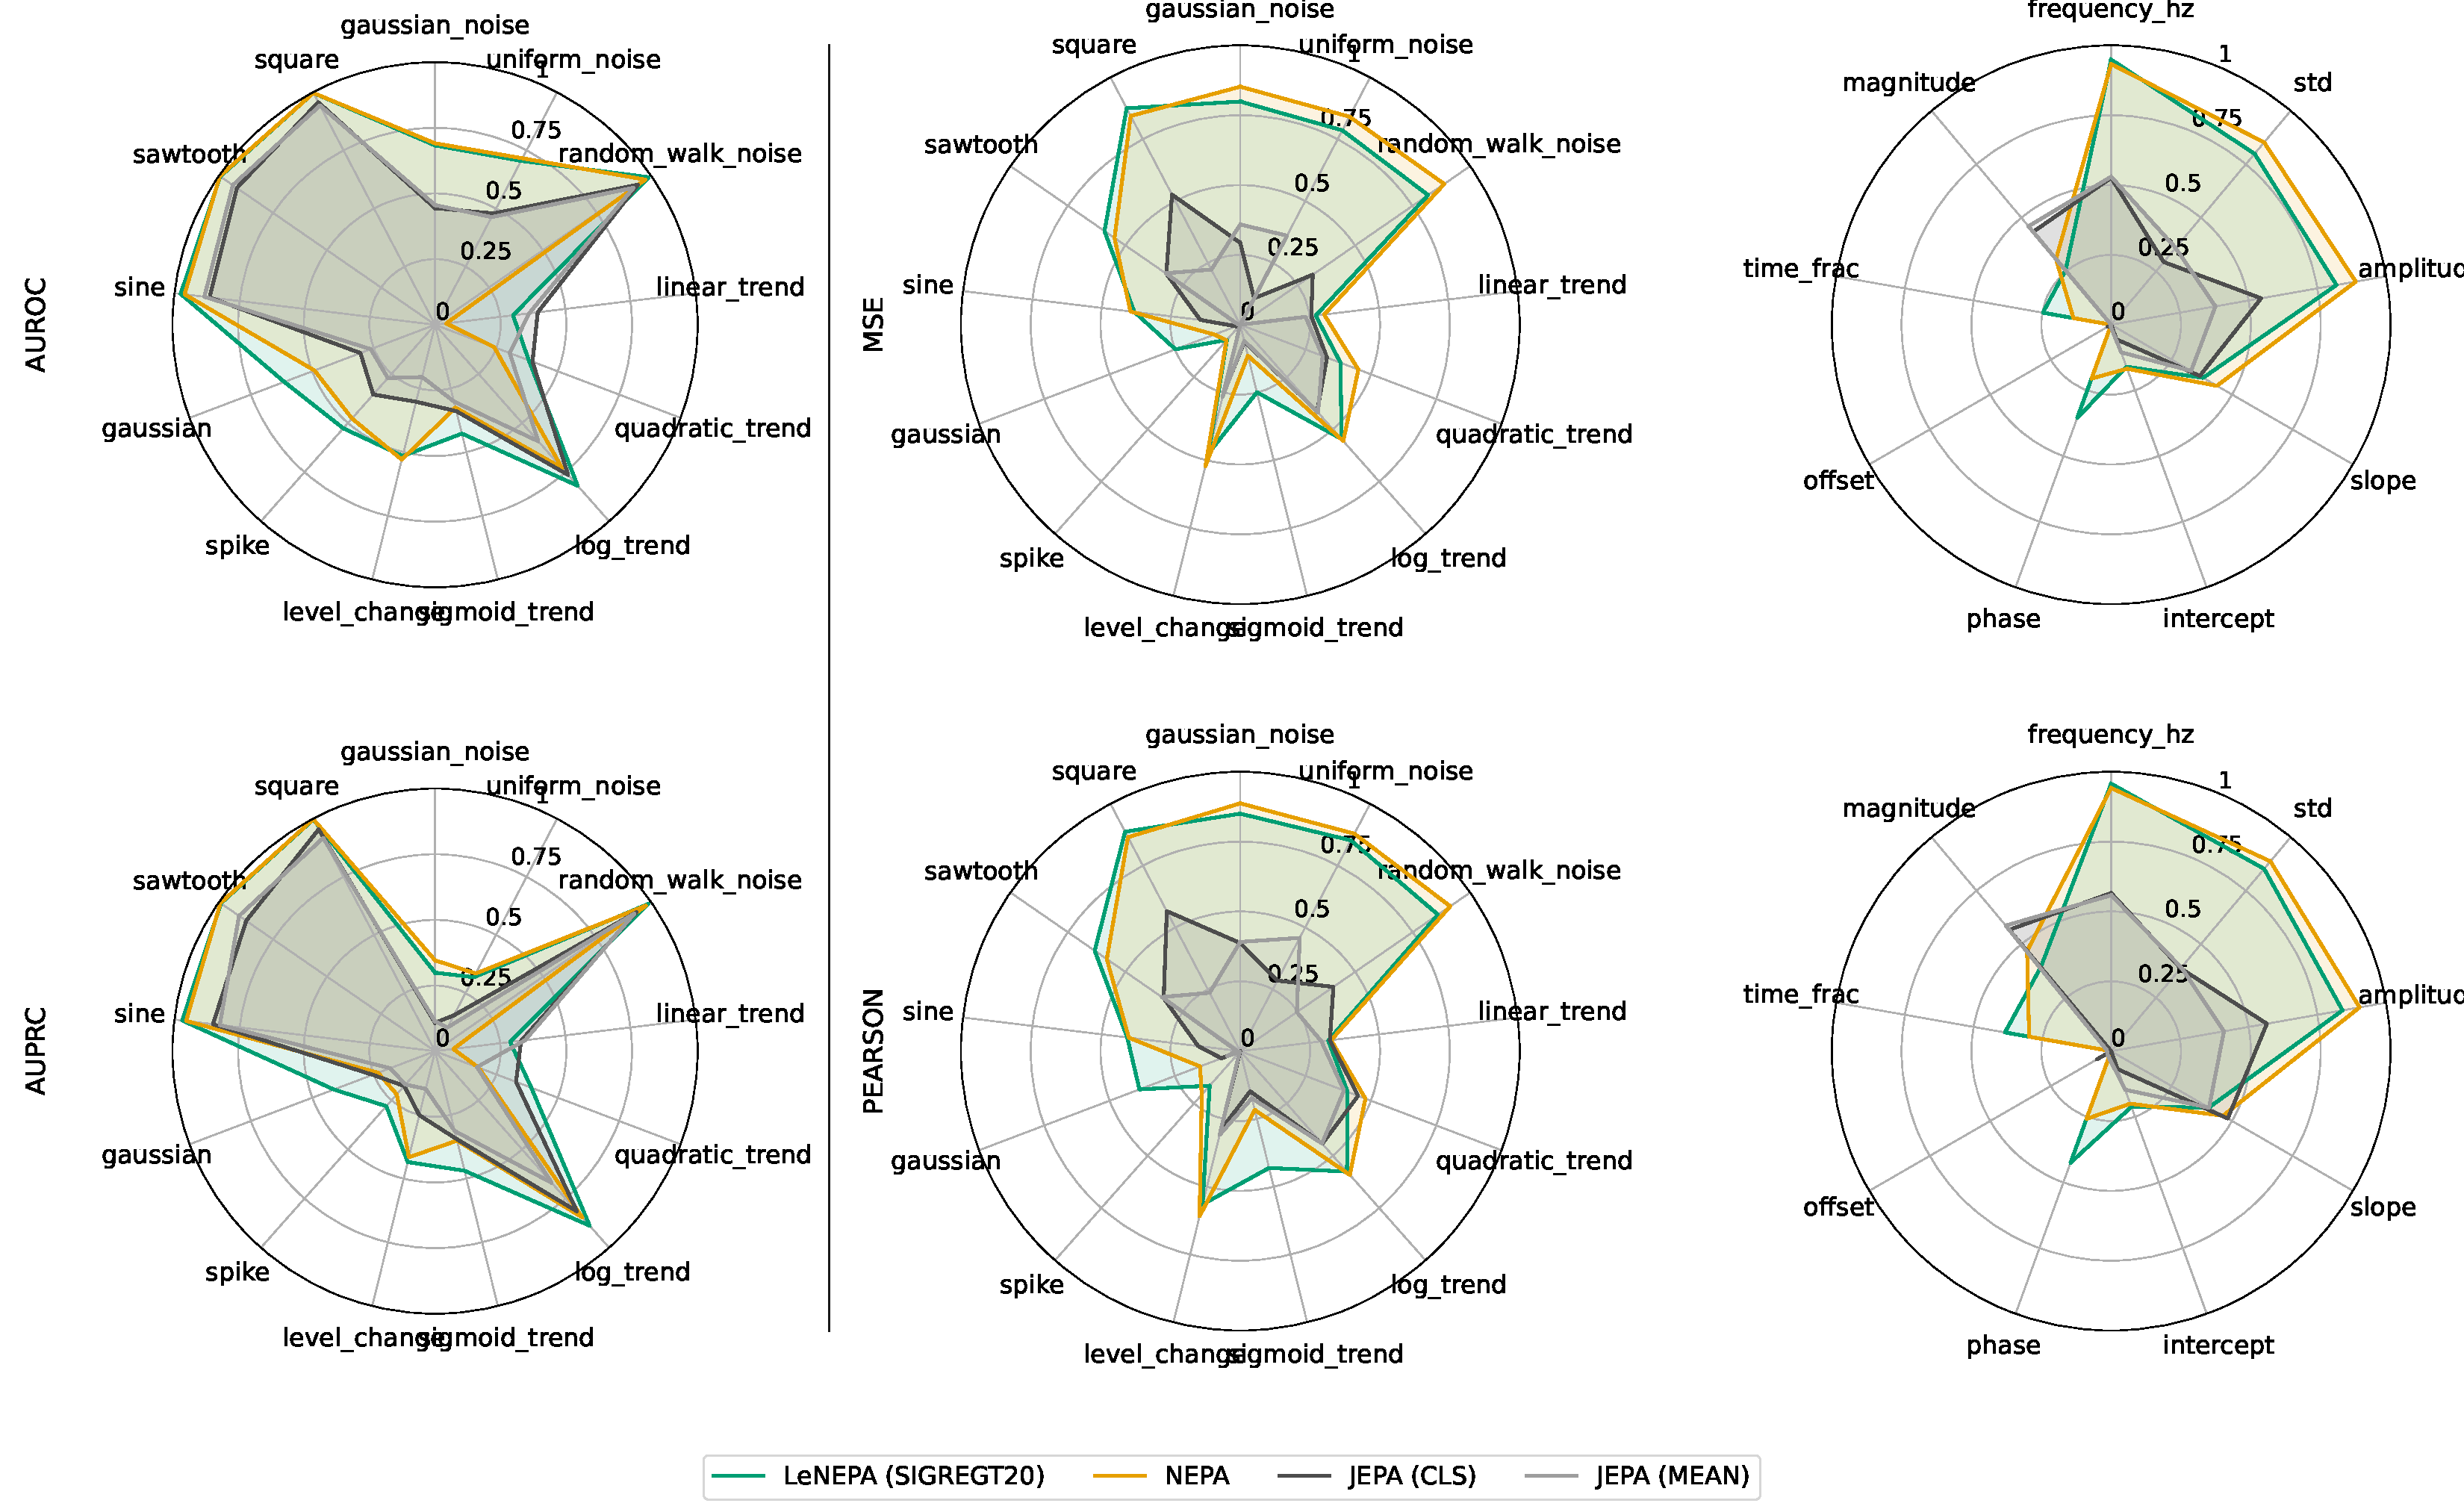
\includegraphics[width=\textwidth,height=0.40\textheight,keepaspectratio]{figures/aionoscope_balanced_basic_components_combined_radar_grid.pdf}
  \caption{Balanced sampler (uniform component weights).}
  \label{fig:aionoscope_balanced_basic_components_combined_radar_grid}
\end{subfigure}

\vspace{0.75em}

\begin{subfigure}{\textwidth}
  \centering
  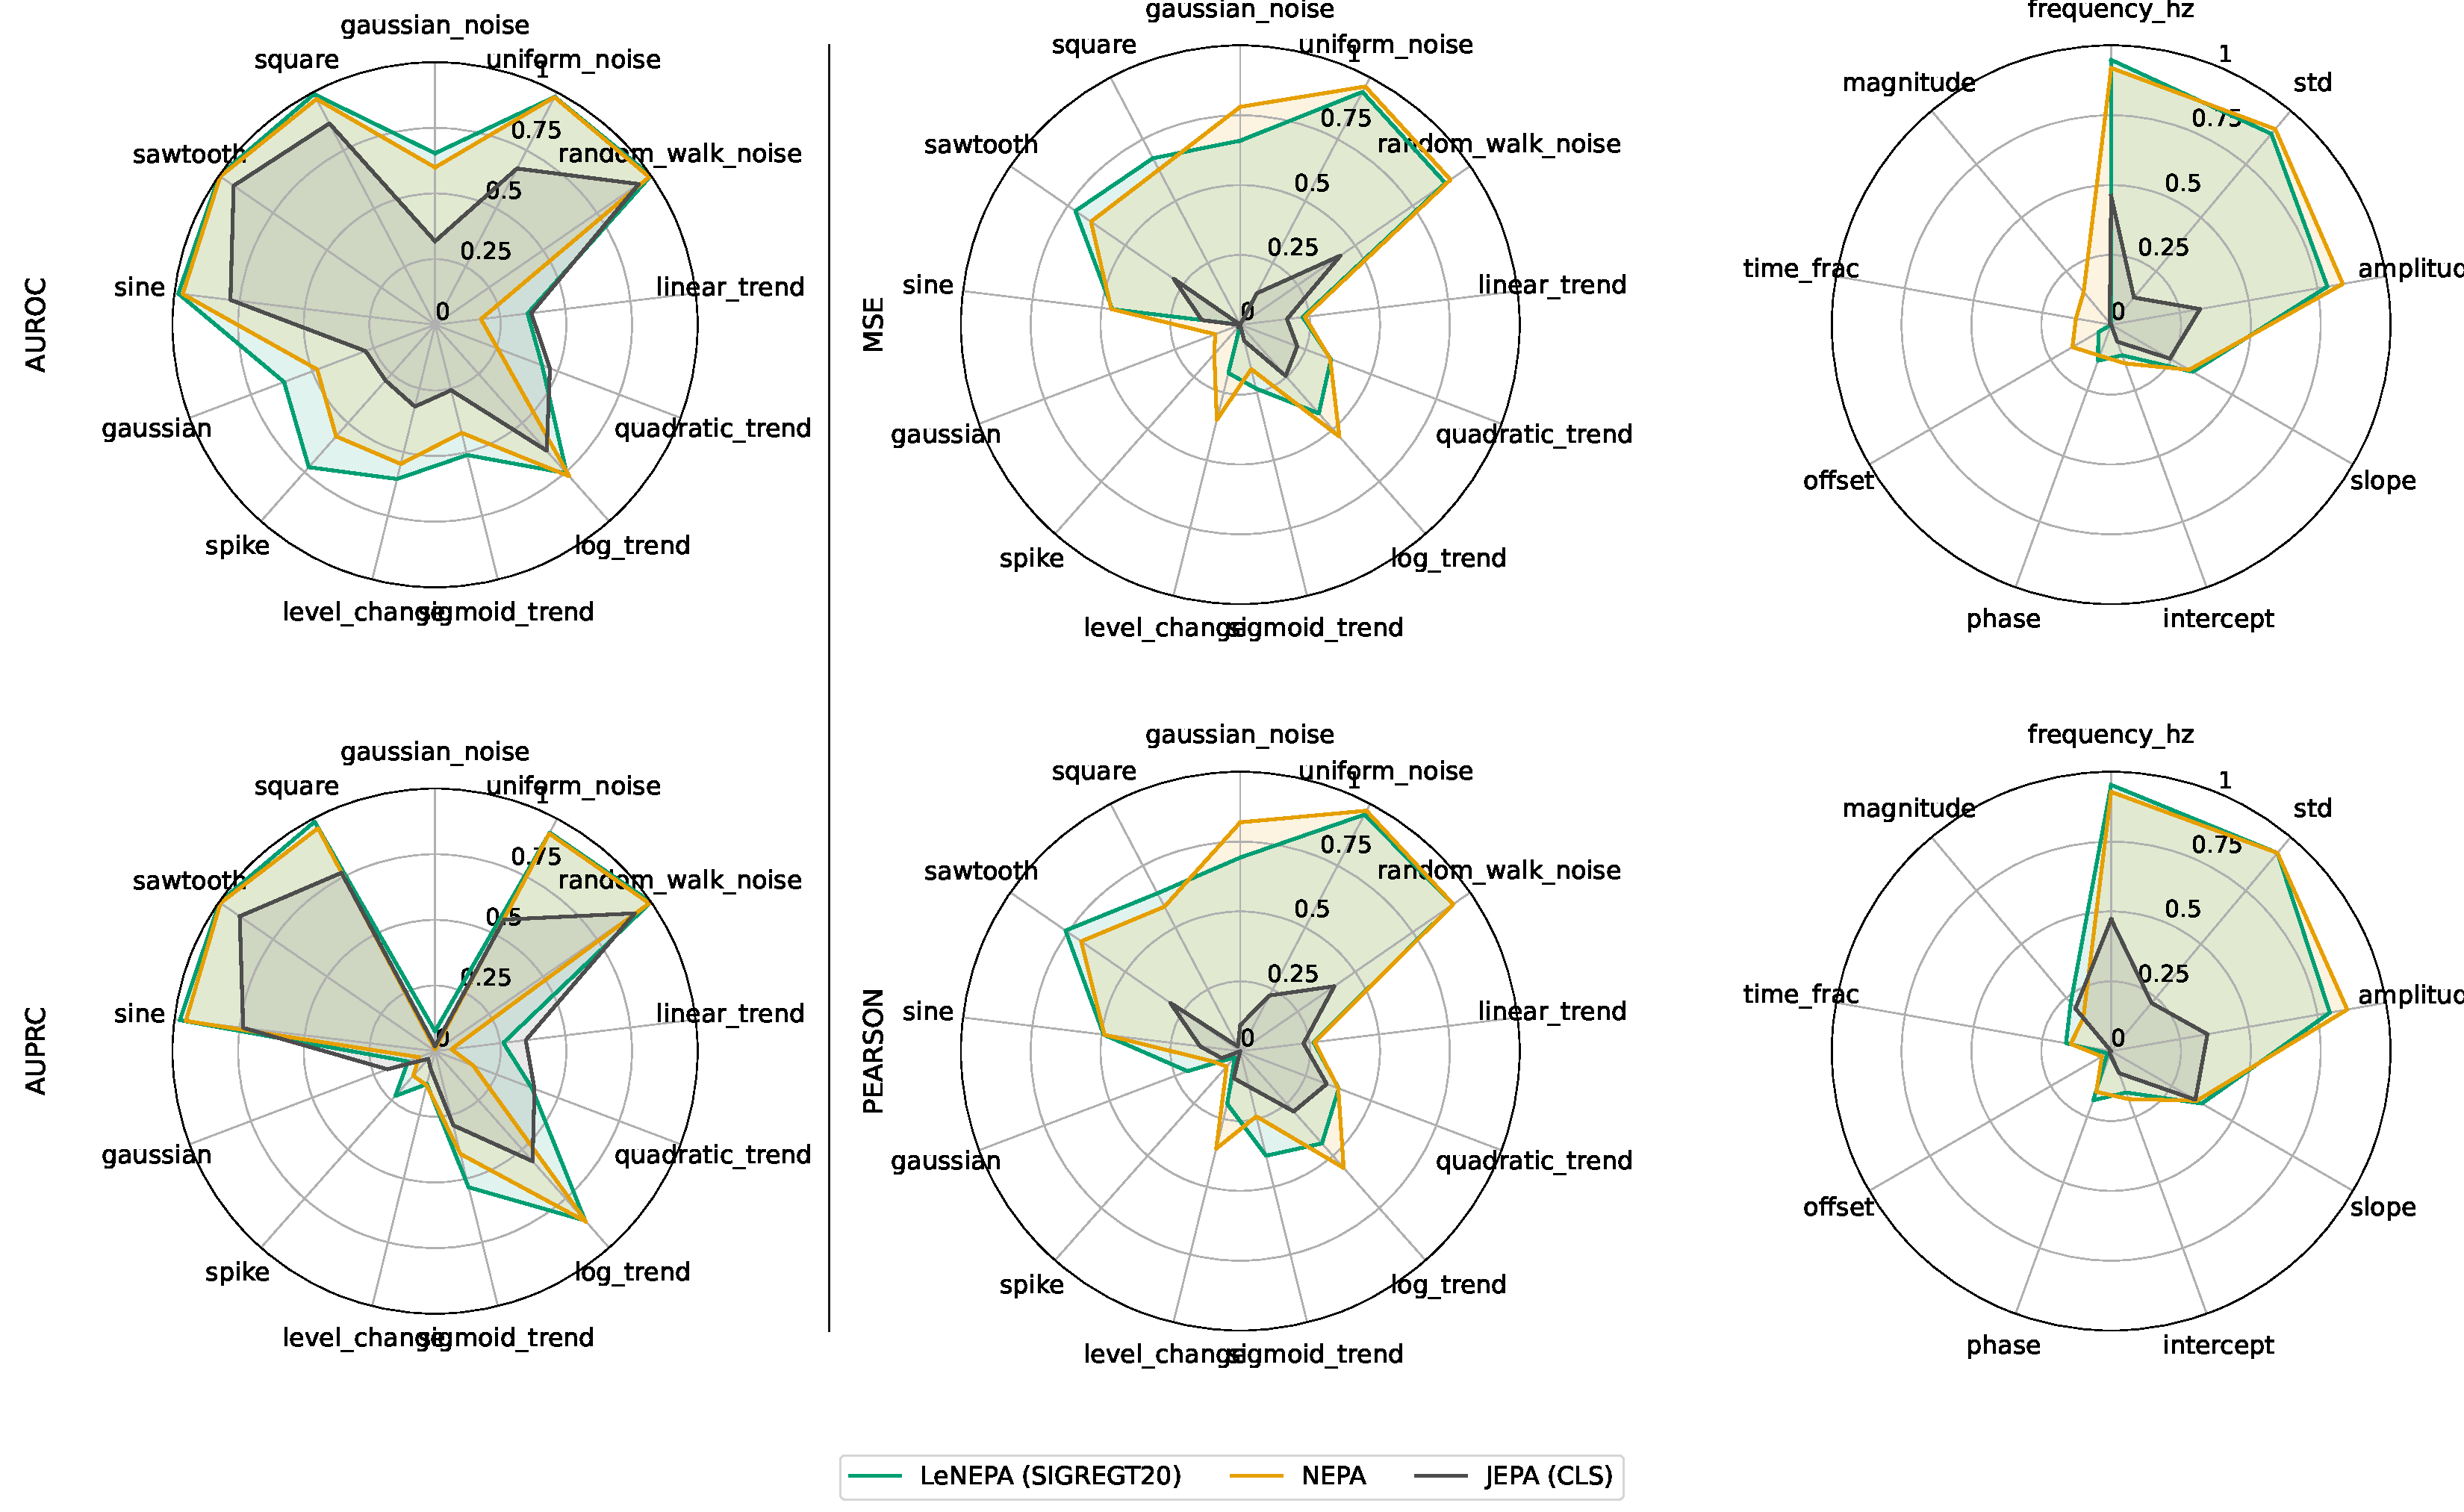
\includegraphics[width=\textwidth,height=0.40\textheight,keepaspectratio]{figures/aionoscope_combined_radar_grid.pdf}
  \caption{Imbalanced sampler with rare components.}
  \label{fig:aionoscope_combined_radar_grid}
\end{subfigure}

\caption{Aionoscope \emph{basic-components} signatures on (a) balanced and (b) imbalanced samplers. Panel (a) includes four objectives (LeNEPA T20, NEPA, JEPA CLS, JEPA MEAN); panel (b) includes LeNEPA T20, NEPA, and JEPA CLS. Left column: per-signal categorical improvements in best-layer AUROC (top) and AUPRC (bottom). Middle and right columns: dense improvements for MSE (top row) and Pearson (bottom row), aggregated by \texttt{target\_signal} families (middle) and by \texttt{target\_metric} types with $>1$ targets (right). For each signal/target we compute a step-$0$ normalized improvement between step $0$ and step $20{,}000$ using the best layer (layers $0$--$8$, selected independently at each step) and clamp scores to $[0,1]$. Dense panels report the median across targets within each group. Higher scores indicate larger relative improvements.}
\end{figure*}

\subsection{Experiment Matrix}
\label{sec:appendix_experiments_matrix}

Across two datasets (Aionoscope \emph{basic-components} and PTB-XL), we compare three families of self-supervised pretraining objectives:
\begin{itemize}
  \item \textbf{JEPA:} an augmentation-based JEPA baseline, evaluated with both CLS-token and mean-pooling readouts.
  \item \textbf{NEPA:} a next-embedding prediction baseline stabilized with stop-gradient (mean pooling).
  \item \textbf{LeNEPA:} our SIGReg-stabilized NEPA variant (mean pooling; no stop-gradient). We report two representative settings: (i) \texttt{T20 L0-8}, which uses temporal SIGReg with $\lambda_{\text{T}}=20$ applied to layers 0~(embedding) and 8~(last transformer layer); and (ii) \texttt{BRI20 L0-8}, which combines batch-wise, representation-level, and innovation SIGReg with $\lambda_{\text{B}}=\lambda_{\text{R}}=\lambda_{\text{I}}=20$ applied to layers 0~(embedding) and 8~(last transformer layer).
\end{itemize}
Appendix~\ref{sec:appendix_sigreg} defines the exact SIGReg placements and hyperparameters for these LeNEPA variants.
For NEPA/LeNEPA we additionally ablate the effect of the projector head by running each configuration with and without projection (controlled by \texttt{use\_projector}), yielding $8$ runs per dataset and $16$ runs total.

\subsection{Summary Plots}
\label{sec:appendix_experiments_summary}

To disentangle gains due to pretraining from the inherent behavior of the randomly initialized tokenizer+backbone (and dataset-specific baseline effects), we primarily report \emph{improvements over step $0$} rather than absolute last-step values.
Figure~\ref{fig:summary_last_step_delta_from_step0_bars} summarizes the best-layer delta between step $20{,}000$ and step $0$, selecting the best layer separately for each metric and step (over layers $0$--$8$). For MSE/MAE, negative values indicate improvement. Absolute last-step values are shown in Figure~\ref{fig:summary_last_step_bars}.

\begin{figure*}[t]
\centering
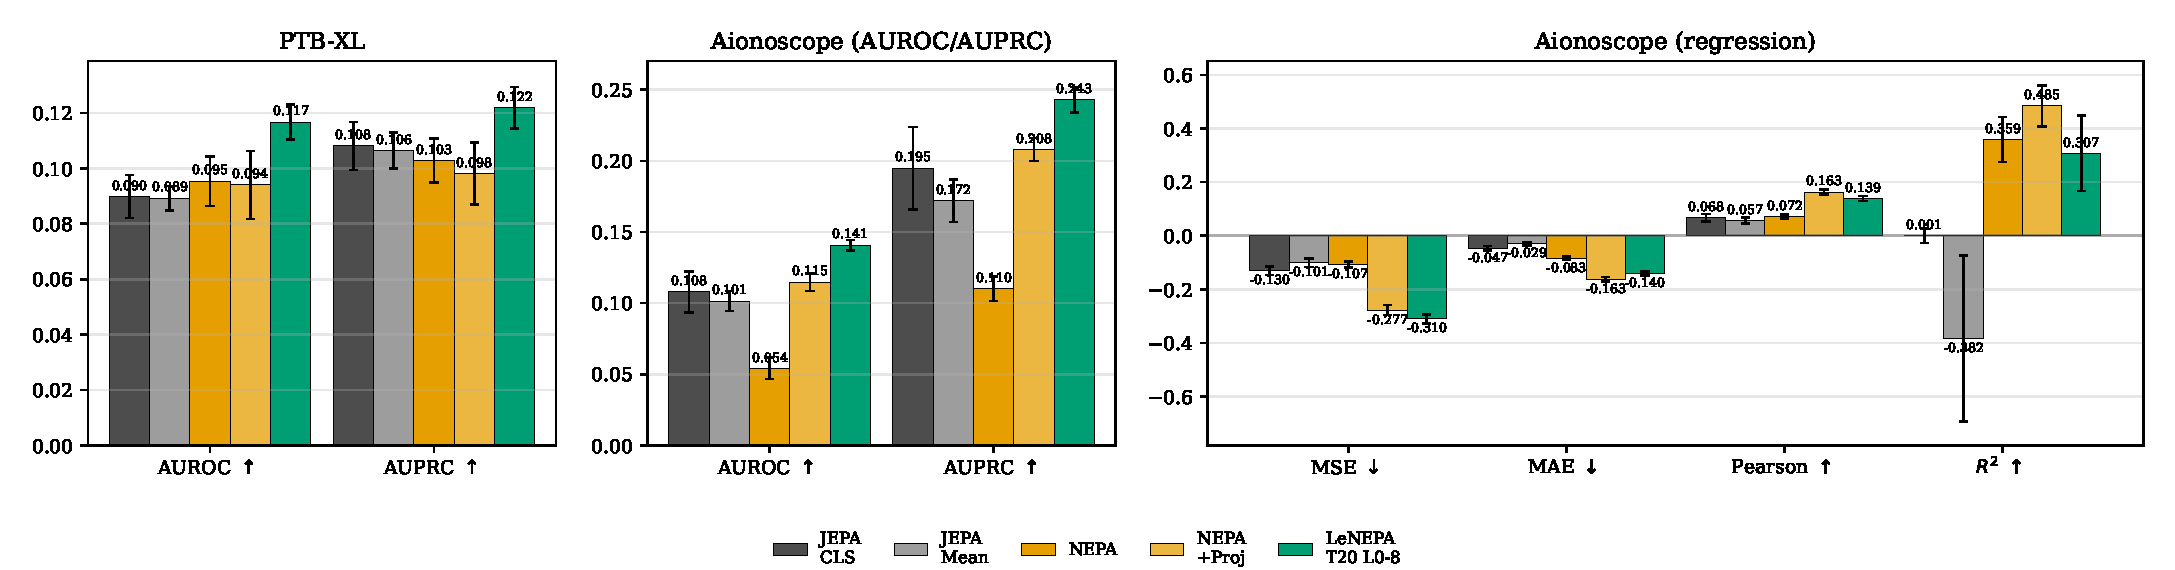
\includegraphics[width=\textwidth]{figures/summary_last_step_delta_from_step0_bars.pdf}
\caption{Last-step (step $20{,}000$) best-layer frozen-backbone probe deltas relative to step $0$ (untrained initialization) on PTB-XL and Aionoscope. For each method and metric, the reported value is the best score over probed layers $0$--$8$, selected separately at step $0$ and at the last step.}
\label{fig:summary_last_step_delta_from_step0_bars}
\end{figure*}

\begin{figure*}[t]
\centering
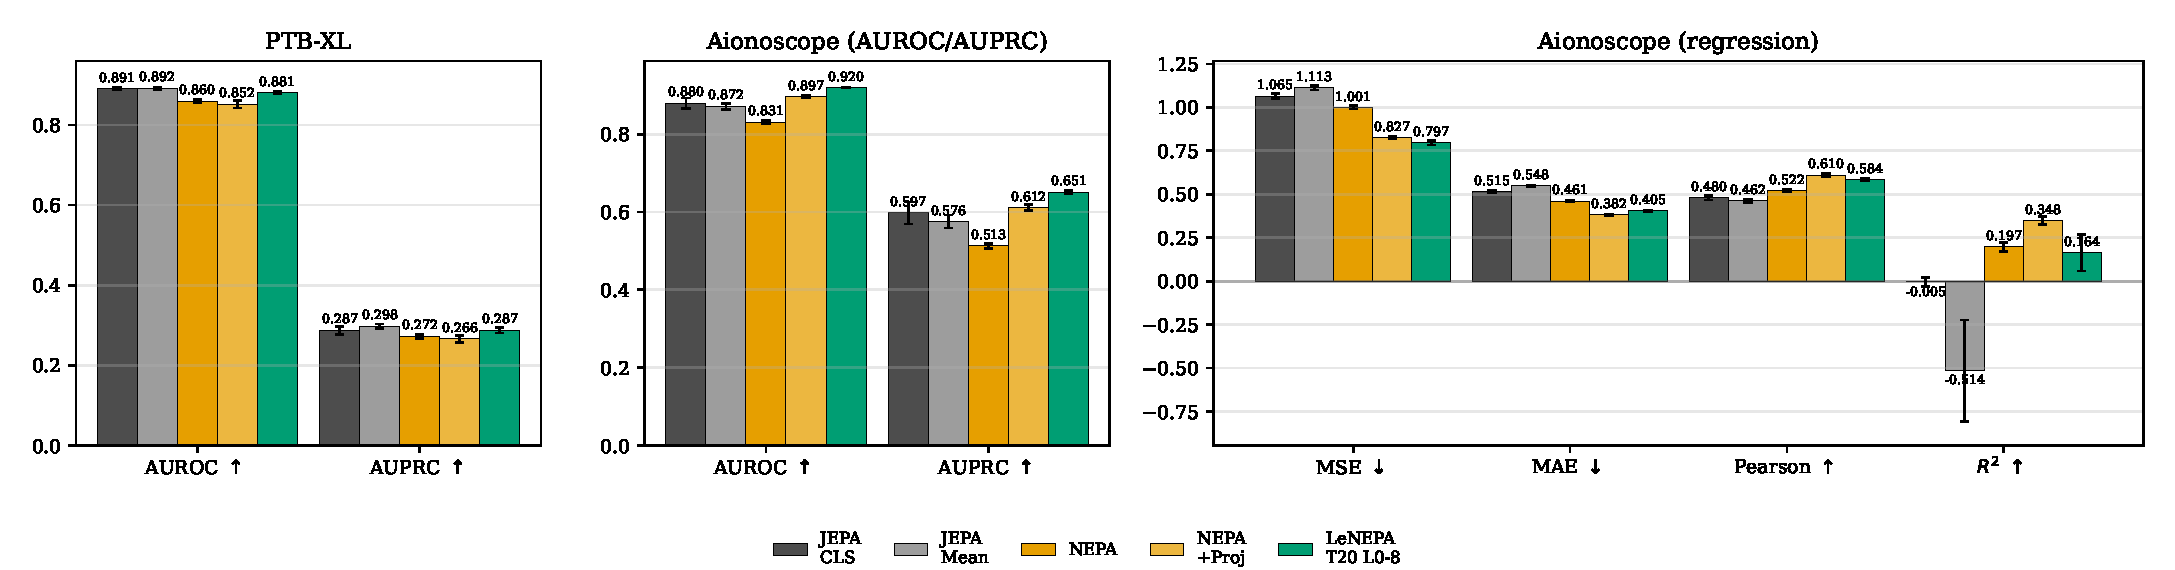
\includegraphics[width=\textwidth]{figures/summary_last_step_bars.pdf}
\caption{Absolute last-step (step $20{,}000$) best-layer frozen-backbone probe performance on PTB-XL and Aionoscope. Bars show macro AUROC/AUPRC for both datasets and MSE/MAE/Pearson/$R^2$ for Aionoscope. For each method and metric, the reported value is the best score over probed layers $0$--$8$.}
\label{fig:summary_last_step_bars}
\end{figure*}

\subsection{Projector Ablation}
\label{sec:appendix_experiments_projector}

We ablate the LeNEPA/NEPA projector $h_{\psi}$ (Appendix~\ref{sec:appendix_projector}), inspired by Guillotine Regularization~\citep{bordes2022guillotine}, by comparing variants that compute the predictive loss (and, when applicable, SIGReg) in a projected space (\texttt{use\_projector=true}) versus directly in backbone token space (\texttt{use\_projector=false}).
Table~\ref{tab:projector_ablation_last_step} reports last-step best-layer probe metrics for no-projector ($-$) versus projector ($+$) variants.

\begin{table}[t]
\centering
\scriptsize
\caption{Projector ablation (NEPA / LeNEPA): best-layer value at the last \emph{common} offline-probe eval step across seeds and projector toggles, aggregated across seeds as $\mathrm{median}(\mathrm{std})$ (ddof=1; std shown in $10^{-3}$ units). Each cell reports $-\mathrm{Proj} / +\mathrm{Proj}$; within each pair, the better value by median is bold (higher is better for AUROC / AUPRC / Pearson / $R^2$; lower is better for MSE / MAE).}
\label{tab:projector_ablation_last_step}

\setlength{\tabcolsep}{3pt}
\renewcommand{\arraystretch}{1.15}
\resizebox{\linewidth}{!}{%
\begin{tabular}{lllrrrrrr}
\toprule
& & & \multicolumn{2}{c}{Classification} & \multicolumn{4}{c}{Dense regression} \\
\cmidrule(lr){4-5}\cmidrule(lr){6-9}
dataset & model & config & AUROC & AUPRC & MSE & MAE & Pearson & $R^2$ \\
\midrule
\multirow{3}{*}{PTB-XL} & NEPA &  & \textbf{0.860(3)} / 0.852(9) & \textbf{0.272(5)} / 0.266(8) & \multicolumn{4}{c}{\textemdash} \\
& LeNEPA & T20 L0-8 & 0.864(4) / \textbf{0.881(3)} & 0.259(4) / \textbf{0.287(6)} & \multicolumn{4}{c}{\textemdash} \\
& LeNEPA & BRI20 L0-8 & 0.832(7) / \textbf{0.863(4)} & 0.245(5) / \textbf{0.278(6)} & \multicolumn{4}{c}{\textemdash} \\
\midrule
\multirow{3}{*}{Aionoscope} & NEPA &  & 0.831(4) / \textbf{0.897(2)} & 0.513(6) / \textbf{0.612(7)} & 1.001(9) / \textbf{0.827(8)} & 0.461(3) / \textbf{0.382(3)} & 0.522(4) / \textbf{0.610(7)} & 0.197(24) / \textbf{0.348(23)} \\
& LeNEPA & T20 L0-8 & 0.848(3) / \textbf{0.920(1)} & 0.588(11) / \textbf{0.651(4)} & 0.886(32) / \textbf{0.797(12)} & 0.449(18) / \textbf{0.405(4)} & 0.519(17) / \textbf{0.584(6)} & -0.214(138) / \textbf{0.164(105)} \\
& LeNEPA & BRI20 L0-8 & 0.868(6) / \textbf{0.902(1)} & 0.567(9) / \textbf{0.608(3)} & 0.975(10) / \textbf{0.834(10)} & 0.502(4) / \textbf{0.396(4)} & 0.488(7) / \textbf{0.590(6)} & -0.767(337) / \textbf{-0.437(228)} \\
\bottomrule
\end{tabular}
} % resizebox
\end{table}


Across the $24$ metric comparisons in Table~\ref{tab:projector_ablation_last_step} (two PTB-XL metrics and six Aionoscope metrics for each of three configurations), projector-enabled variants are better in $22/24$ cases.
The only exception is NEPA on PTB-XL classification, where the no-projector variant is slightly better.
Therefore, in the remainder of this work we use LeNEPA \emph{only} with the projector enabled, and report both NEPA and NEPA~+Proj for clarity.

\subsection{SIGReg Component Ablations}
\label{sec:appendix_experiments_sigreg_component_ablations}

To isolate the effect of each SIGReg placement (Appendix~\ref{sec:appendix_sigreg}), we run LeNEPA with exactly one SIGReg component enabled at scale $20$ (projector enabled; \texttt{pred\_depth=0}; seed $0$) while keeping the predictive loss $\mathcal{L}_{\text{pred}}$ unchanged.
Concretely, using the notation from Appendix~\ref{sec:appendix_sigreg}, we denote by $u^{(\ell)}\in\mathbb{R}^{B\times T\times d}$ the projected patch-token embeddings at layer $\ell$ (after the optional projector $h_{\psi}$), and we set $\lambda_{\text{pred}}=1$ and enable exactly one of $\{\lambda_{\text{B}},\lambda_{\text{T}},\lambda_{\text{R}},\lambda_{\Delta},\lambda_{\text{BT}}\}$ at value $20$, with all other SIGReg scales set to $0$ in Eq.~\eqref{eq:sigreg_total}.
We use $\mathcal{L}_{\text{B}}=\mathcal{L}_{\text{T}}=\mathcal{L}_{\Delta}=\mathcal{L}_{\text{BT}}=\{0,8\}$ and $\mathcal{L}_{\text{R}}=\{8\}$, matching the layer choices in the main matrix.

\paragraph{Single-component variants.}
\begin{itemize}
  \item \textbf{\texttt{B20} (batch-wise SIGReg).} We regularize the distribution across the batch at each time index (Eq.~\eqref{eq:sigreg_batch}), encouraging non-collapsed embeddings across samples while preserving the temporal structure within each sample.
  \item \textbf{\texttt{T20} (temporal SIGReg).} We regularize the distribution across time for each sample (Eq.~\eqref{eq:sigreg_time}), explicitly discouraging per-sample temporal collapse where token embeddings become nearly constant over the time axis.
  \item \textbf{\texttt{R20} (representation-level SIGReg).} We apply SIGReg to pooled per-layer sequence representations $r^{(\ell)}$ (Eq.~\eqref{eq:sigreg_rep}), using the same readout as for linear probing. In our setup this is mean pooling over patch tokens, $r^{(\ell)}_b=\frac{1}{T}\sum_{t=1}^{T}u^{(\ell)}_{b,t}$. This placement is the closest to the original LeJEPA use of SIGReg~\citep{balestriero2025lejepa}, which regularizes a single representation vector per sample/view rather than token sequences.
  \item \textbf{\texttt{I20} (innovation SIGReg).} We apply SIGReg to innovations $\Delta u^{(\ell)}_{b,t}=u^{(\ell)}_{b,t+1}-u^{(\ell)}_{b,t}$ (Eq.~\eqref{eq:sigreg_innov_def}--\eqref{eq:sigreg_innov}), regularizing dynamics (temporal differences) rather than absolute token values.
  \item \textbf{\texttt{BT20} (batch-time SIGReg).} We flatten batch and time and apply SIGReg to the joint set of tokens per layer (Eq.~\eqref{eq:sigreg_batch_time}). Relative to \texttt{B20} and \texttt{T20}, this is a more relaxed axis-agnostic constraint: it enforces global non-collapse across all token instances while avoiding explicit per-time-index (\texttt{B20}) or per-sample temporal (\texttt{T20}) regularization, serving as a check that our conclusions are not driven by over-regularizing along a specific axis.
\end{itemize}

\paragraph{Layer placement relative to $\mathcal{L}_{\text{pred}}$.}
In our main LeNEPA setup, the prediction loss $\mathcal{L}_{\text{pred}}$ (Eq.~\eqref{eq:lenepa_pred}) aligns predicted tokens from the top backbone layer ($\ell=8$) with next-step targets taken from the tokenizer embedding layer ($\ell=0$).
We observed that applying SIGReg to both sides of this regression (i.e., regularizing layers $\{0,8\}$) yields more transferable frozen-backbone representations in most cases than applying SIGReg only on the prediction side (layer $8$).
In contrast, applying SIGReg only to the embedding targets (layer $0$) yields substantially weaker transfer.
More generally, applying SIGReg to layers that do not participate in $\mathcal{L}_{\text{pred}}$ (e.g., intermediate layers when targets are taken from $\ell=0$) leads to collapse or severely degraded transfer.
We omit plots for these additional ablations due to space constraints.
We hypothesize that SIGReg is most effective when it directly counterbalances the prediction objective in the same embedding space as $\mathcal{L}_{\text{pred}}$, rather than regularizing features that are not directly tied to the regression targets.

Finally, we compare these single-component variants to the multi-term reference configuration \texttt{BRI20} used in the main matrix ($\lambda_{\text{B}}=\lambda_{\text{R}}=\lambda_{\Delta}=20$ with the layer sets above).
Figure~\ref{fig:sigreg_component_ablations_dynamics} reports best-layer transfer dynamics (over layers $0$--$8$).
The top row shows AUROC/AUPRC for PTB-XL and Aionoscope, while the bottom row shows Aionoscope dense-target metrics (MSE/MAE/Pearson/$R^2$).
In our setup, temporal SIGReg is the only single-component placement that consistently yields sustained improvements in frozen-backbone transfer performance across both datasets.

\begin{figure*}[t]
\centering
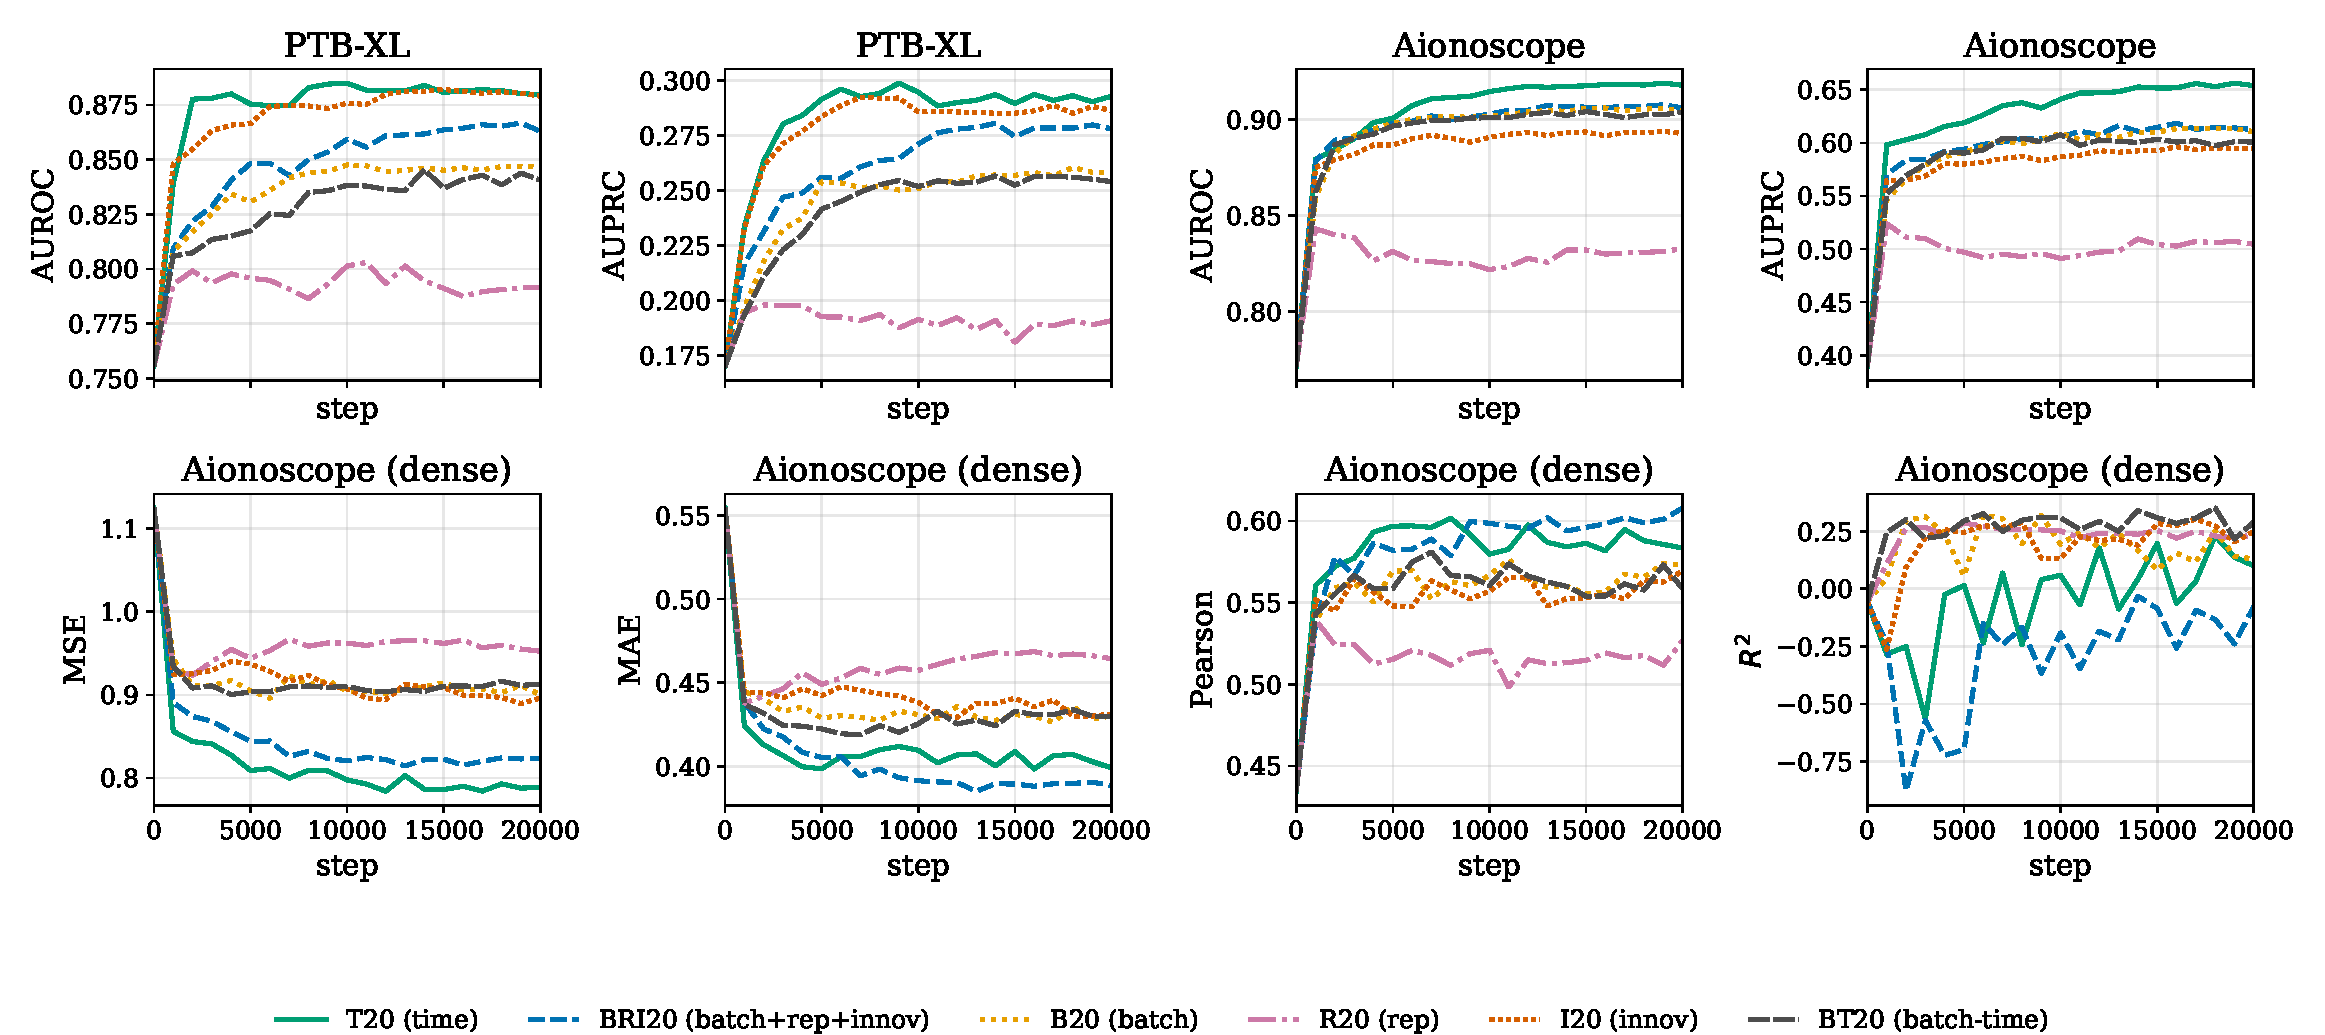
\includegraphics[width=\textwidth]{figures/sigreg_component_ablations_dynamics.pdf}
\caption{SIGReg component ablations (seed $0$ only; projector enabled): best-layer transfer dynamics for time-only (\texttt{T20}), batch-only (\texttt{B20}), representation-only (\texttt{R20}), innovation-only (\texttt{I20}), batch-time-only (\texttt{BT20}), and the multi-term reference configuration (\texttt{BRI20}). Top row: classification AUROC/AUPRC for PTB-XL and Aionoscope. Bottom row: Aionoscope dense-target metrics (MSE/MAE/Pearson/$R^2$), where lower is better for MSE/MAE. Best layer is selected independently at each step (over layers $0$--$8$).}
\label{fig:sigreg_component_ablations_dynamics}
\end{figure*}

\subsection{Aionoscope Dense Target Training Dynamics}
\label{sec:appendix_experiments_aionoscope_dense_dynamics}

Figure~\ref{fig:aionoscope_dynamics_best_layer_dense} reports training dynamics for dense regression targets on the Aionoscope \emph{basic-components} benchmark.
For each metric and each offline-probe evaluation step, we plot the best-layer value over probed layers $0$--$8$.

\begin{figure*}[t]
\centering
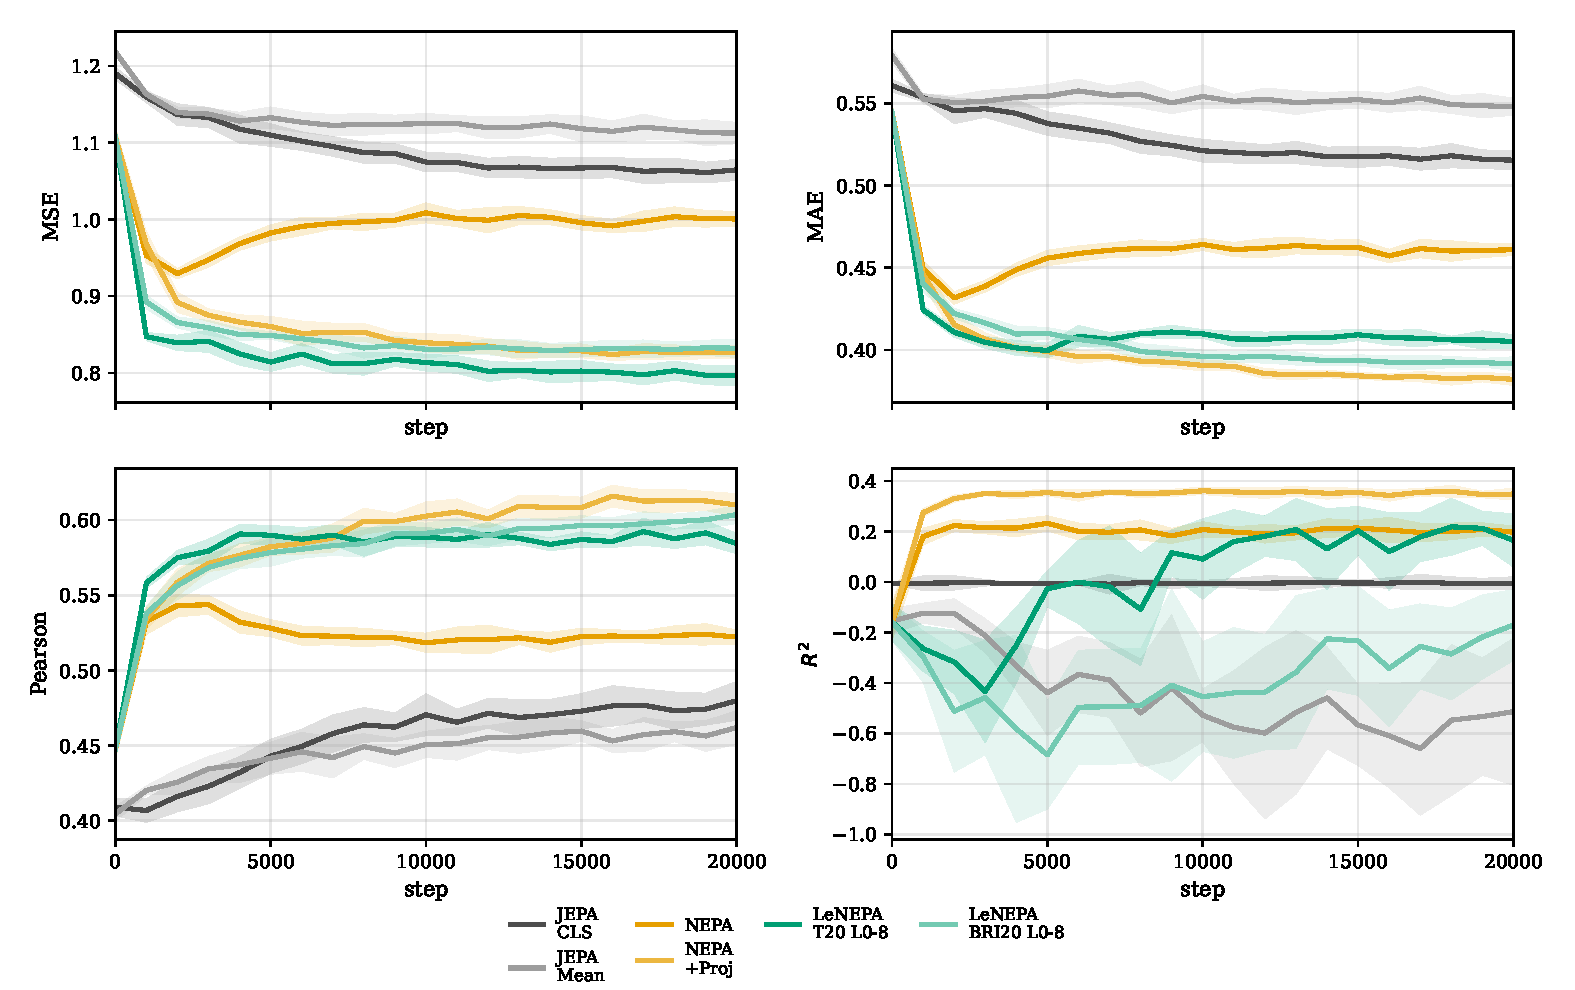
\includegraphics[width=\textwidth]{figures/aionoscope_dynamics_best_layer_dense.pdf}
\caption{Aionoscope \emph{basic-components} dense-target dynamics: best-layer over layers $0$--$8$ frozen-backbone probe performance over training steps for MSE/MAE/Pearson/$R^2$.}
\label{fig:aionoscope_dynamics_best_layer_dense}
\end{figure*}

\subsection{JEPA Masking Fragility}
\label{sec:appendix_experiments_jepa_masking_fragility}

JEPA relies on a masking-based view construction controlled by a keep-ratio range, $\rho \sim \mathrm{Uniform}(\rho_{\min}, \rho_{\max})$, which determines the fraction of tokens retained in the context view.
To illustrate the sensitivity of augmentation-driven SSL in time series, we rerun the PTB-XL JEPA (CLS) configuration with two alternative keep-ratio ranges:
(i) a more aggressive masking regime $(\rho_{\min},\rho_{\max})=(0.05,0.10)$ and
(ii) a lighter masking regime $(\rho_{\min},\rho_{\max})=(0.30,0.40)$, compared to the baseline $(0.15,0.25)$ used throughout the paper.
All other hyperparameters, including the $20{,}000$-step fixed-horizon protocol and the layer-wise offline probing setup, are kept identical. The resulting best-layer AUROC/AUPRC training dynamics are shown in Figure~\ref{fig:ptbxl_jepa_masking_fragility_dynamics}.
As we can see, changing the augmentation parameters by just $2$--$3\times$ leads to a significant degradation in the representation quality.

\begin{figure*}[t]
\centering
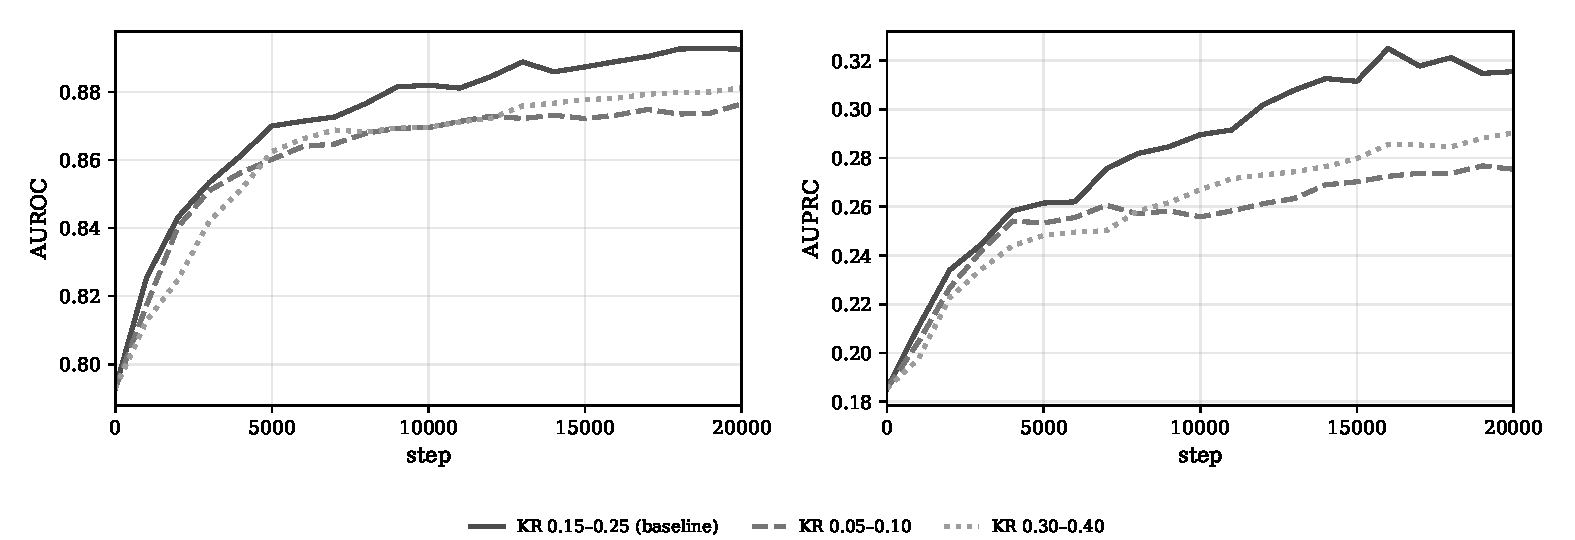
\includegraphics[width=\textwidth]{figures/ptbxl_jepa_masking_fragility_dynamics.pdf}
\caption{PTB-XL JEPA masking fragility (seed $0$ only): best-layer AUROC/AUPRC dynamics under different keep-ratio ranges (selected over layers $0$--$8$ at each step).}
\label{fig:ptbxl_jepa_masking_fragility_dynamics}
\end{figure*}
